\section{Active Learning for Imbalanced Data Classification}
\label{al_for_imbalanced_data}
As outlined in Section~\ref{sec:background}, active learning is primarily considered as a technique to reduce the number of training samples that need to be labeled for a classification task. From a traditional perspective, the active learner has access to a vast pool of unlabeled examples, and it aims to make a clever choice to select the most informative example to obtain its label. However, even in the cases where the labels of training data are already available, active learning can still be leveraged to obtain the informative examples through training sets \cite{Schohn_2000,Bordes_2005,Huang_2006}. For example, in large-margin classifiers such as Support Vector Machines (SVM), the \textit{informativeness} of an example is synonymous with its distance to the hyperplane. The farther an example is to the hyperplane, the more the learner is confident about its true class label; hence there is little, if any, benefit that the learner can gain by asking for the label of that example. On the other hand, the examples close to the hyperplane are the ones that yield the most information to the learner. Therefore, the most commonly used active learning strategy in SVMs is to check the distance of each unlabeled example to the hyperplane and focus on the examples that lie closest to the hyperplane, as they are considered to be the most informative examples to the learner~\cite{tong02svm}.

\begin{figure}[t!]
    \centering
        \scalebox{0.37}{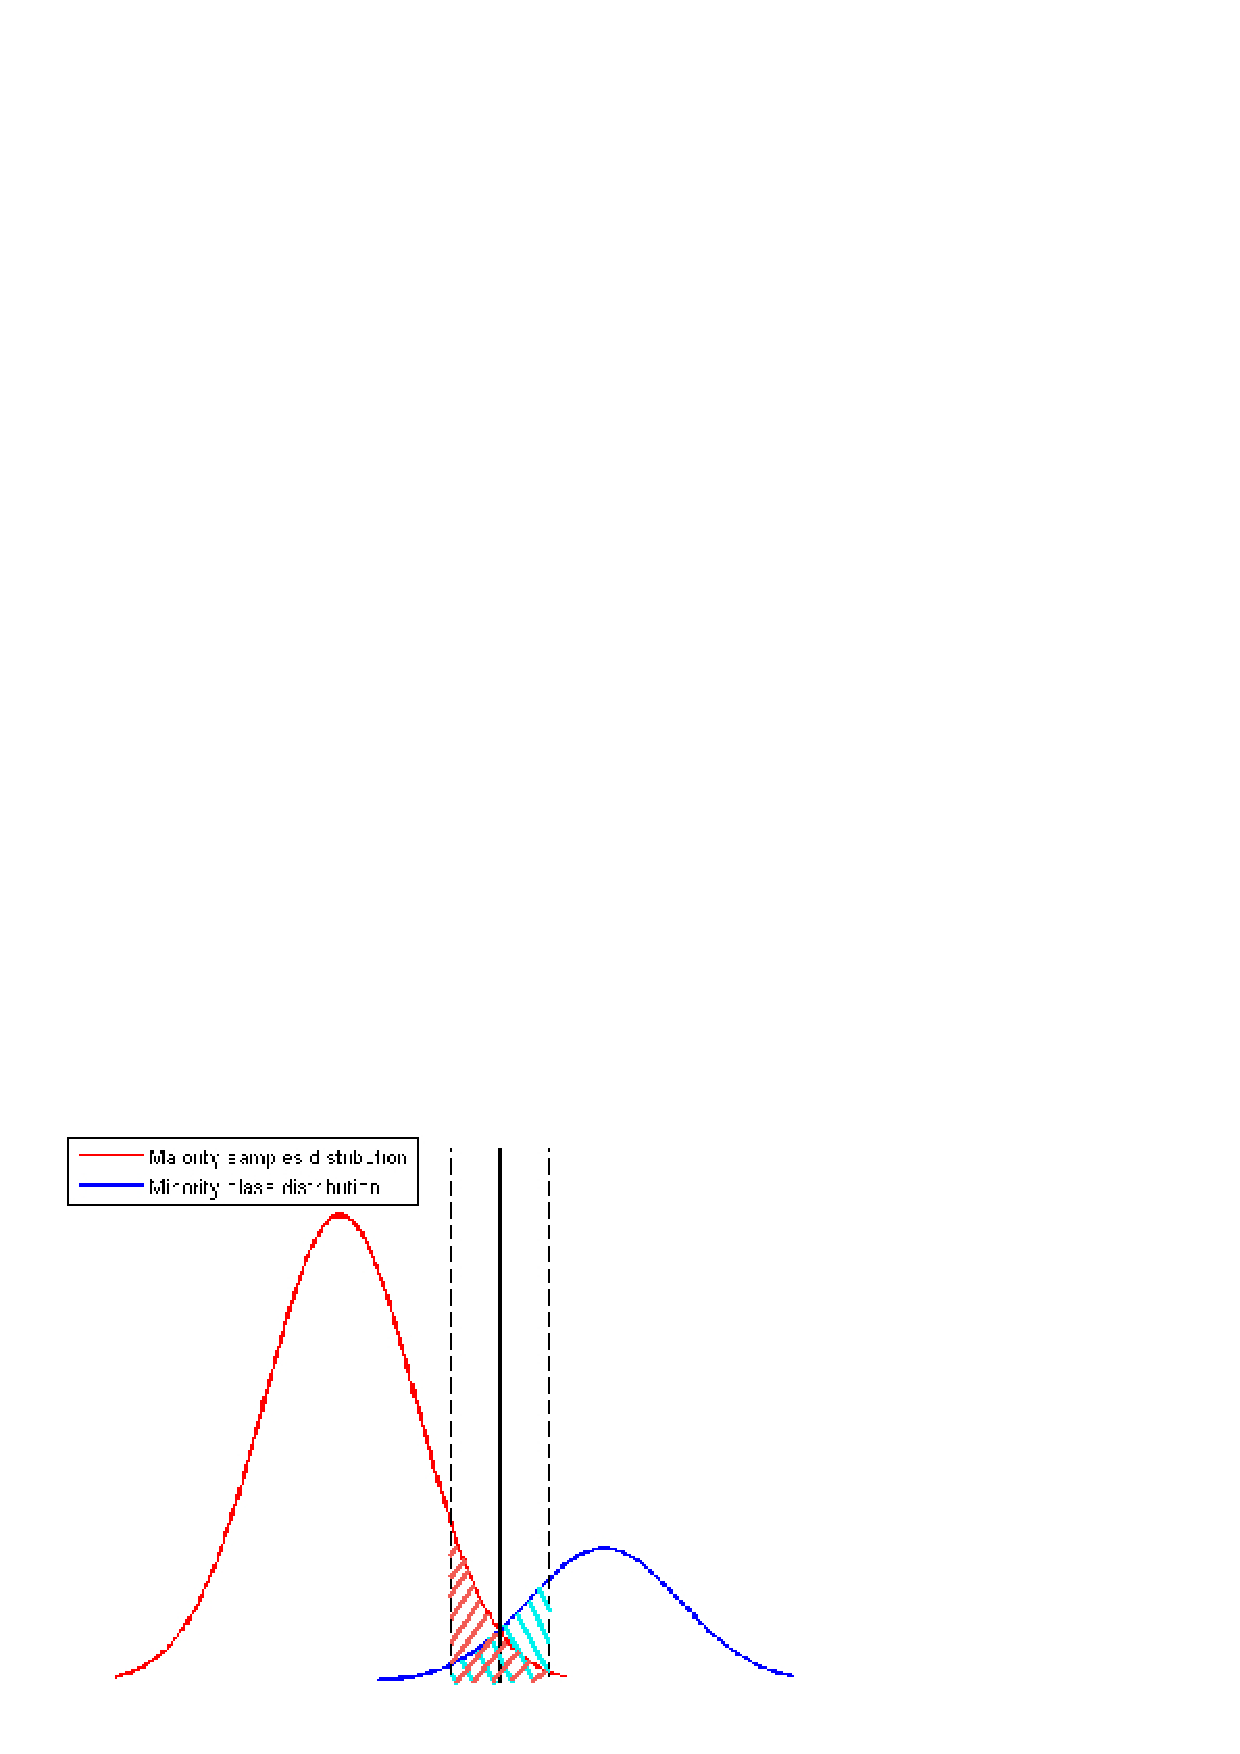
\includegraphics{Figures/lotb/al-imb-shade.pdf}}
    \caption{Data within the margin is less imbalanced than the entire data.}
    \label{fig:alimbshade}
\end{figure}

The strategy of selecting examples within the margin also strongly addresses the problems that arise from imbalanced classes.  Consider the class distributions of an imbalanced dataset presented in Figure \ref{fig:alimbshade}. The shaded region corresponds to the class distribution of the data within the margin. As shown in the figure, the imbalance ratio of the classes within the margin is much smaller than the class imbalance ratio of the entire dataset. Therefore, any selection strategy that focuses on the examples in the margin most likely ends up with a more balanced class distribution than that of the entire dataset. %Our empirical findings with various type of real-world data confirm that the imbalance ratios of the classes within the margin in real-world data are generally much lower than that of the entire data.

Throughout this section, the discussion is constrained to standard two-class classification problems using Support Vector Machines (SVMs). The next subsection presents a brief overview of SVMs, followed by the working principles of an efficient active learning algorithm in Section \ref{ALpools}. We explain the advantage of using online SVMs with the active sample selection in Section \ref{LASVM}.% In Section \ref{ES}, we then describe an early stopping heuristics for active learning.

\subsection{Support Vector Machines}
\label{SVMs}
Support Vector Machines \cite{Vapnik_1995} are well known for their strong theoretical foundations, generalization performance and ability to handle high dimensional data. In the binary classification setting, let $((x_{1}, y_{1})\cdots(x_{n}, y_{n}))$ be the training dataset where $x_i$ are the feature vectors representing the instances and  $y_i \in (-1,+1)$ be the labels of the instances.  Using the training set, SVM builds an optimum hyperplane -- a linear discriminant in a higher dimensional feature space -- that separates the two classes by the largest margin. This hyperplane is obtained by minimizing the following objective function:
\begin{equation}
\label{svm_primal}
\min_{{\bf{w}, b, \xi_{i}}}\frac{1}{2} {\bf w\cdot w}^T + C\sum_{i=1}^{N}\xi_i  \\
\end{equation}
\begin{equation}
\mbox{subject to}\left\{ \begin{array}{l} \forall i \; y_i({\bf
w}^T{\Phi(x_i)} - b)\geq 1-\xi_{i}\\ \forall i \; \xi_{i} \geq 0
\end{array} \right.
\end{equation}
where \textbf{w} is the norm of the hyperplane, $b$ is the  offset, $y_i$ are the labels, $\Phi(\cdot)$ is the mapping from input space to feature space, and $\xi_i$ are the slack variables that permit the non-separable case by allowing misclassification of training instances. In practice the convex quadratic programming (QP) problem in (\ref{svm_primal}) is solved by optimizing the dual cost function. The dual representation of (\ref{svm_primal}) is given as
\begin{equation}
\label{svm_dual}
\max W(\alpha) \equiv \sum_{i=1}^{N}\alpha_{i} - \frac{1}{2}\sum_{i,j}\alpha_i\alpha_{j}y_{i}y_{j}K({\bf x_i},{\bf x_j}) \\
\end{equation}
\begin{equation}
\mbox{subject to}\left\{ \begin{array}{l} \forall i\; 0 \leq \alpha_i \leq C\\ \sum_{i=1}^{N}\alpha_i y_i=0 \end{array} \right.
\end{equation}
where $y_i$ are the labels, $\Phi(\cdot)$ is the mapping from the input space to the feature space, $K({\bf x_i}, {\bf x_j})=\langle\Phi({\bf x_i}),\Phi({\bf x_j})\rangle$ is the kernel matrix and the $\alpha_i$'s are the \textit{Lagrange multipliers} which are non-zero only for the training instances which fall in the margin. Those training instances are called \textit{support vectors} and they define the position of the hyperplane. After solving the QP problem, the norm of the hyperplane \textbf{w} can be represented as
\begin{equation}
\label{svm_norm}
\textbf{w}=\sum_{i=1}^{n}\alpha_i\Phi(x_i)
\end{equation}

\subsection{Margin-based Active Learning with SVMs}
\label{ALpools}
Note that in (\ref{svm_norm}), only the support vectors affect the SVM solution. This means that if SVM is retrained with a new set of data which only consist of those support vectors, the learner will end up finding the same hyperplane. This emphasizes the fact that not all examples are equally important in training sets. Then the question becomes how to select the most informative examples for labeling from the set of unlabeled training examples. This section focuses on a form of selection strategy called \textit{margin-based active learning}. As was highlighted earlier, in SVMs the most informative example is believed to be the closest one to the hyperplane since it divides the \textit{version space} into two equal parts. The aim is to reduce the version space as fast as possible to reach the solution faster in order to avoid certain \textit{costs} associated with the problem. For the possibility of a non-symmetric version space, there are more complex selection methods suggested by \cite{tong02svm}, but it has been observed that the advantage of those are not significant, considering their high computational costs.

\textbf{Active Learning with Small Pools:}
 The basic working principle of margin-based active learning with SVMs is: $i)$ train an SVM on the existing training data, $ii)$ select the closest example to the hyperplane, and $iii)$ add the new selected example to the training set and train again. In classical active learning \cite{tong02svm}, the search for the most informative example is performed over the entire dataset. Note that, each iteration of active learning involves the recomputation of each training example's distance to the new hyperplane. Therefore, for large datasets, searching the entire training set is a very time consuming and computationally expensive task.

One possible remedy for this performance bottleneck is to use the ``59 trick'' \cite{Smola_2000}, which alleviates a full search through the entire dataset, approximating the most informative examples by examining a small constant number of randomly chosen samples. The method picks $L$ ($L \ll$ \# training examples) random training samples in each iteration and selects the best (closest to the hyperplane) among them. Suppose, instead of picking the closest example among all the training samples $X_N=(x_1, x_2, \cdots ,x_N)$ at each iteration, we first pick a random subset $X_L$, $L\ll N$ and select the closest sample $x_i$ from $X_L$ based on the condition that $x_i$ is among the top $p\%$ closest instances in $X_N$ with probability $(1-\eta)$. Any numerical modification to these constraints can be met by varying the size of $L$, and is independent of $N$. To demonstrate, the probability that at least one of the $L$ instances is among the closest $p$ is $1-(1-p)^L$. Due to the requirement of $(1-\eta)$ probability, we have
\begin{equation}
1-(1-p)^L = 1-\eta
\end{equation}
which follows the solution of $L$ in terms of $\eta$ and $p$
\begin{equation}
L={{\log \eta} \;/\;{\log(1-p)}}
\end{equation}
For example, the active learner will pick one example, with $95\%$ probability, that is among the top $5\%$ closest instances to the hyperplane, by randomly sampling only $\lceil \log(.05)/\log(.95) \rceil = 59$ examples regardless of the training set size. This approach scales well since the size of the subset $L$ is independent of  the training set size $N$, requires significantly less training time and does not have an adverse effect on the classification performance of the learner.

%\begin{figure*}[t]
%    \centering
%        \scalebox{0.34}{\includegraphics{Figures/lotb/rpal.pdf}}
%    \caption{Comparison of PRBEP and g-means of RS, AL(full search) and AL(random pool). The training times of AL(full search) vs. AL(random pool) until saturation in seconds are: 272 vs. 50 (grain), 142 vs. 32 (ship) and 126 vs. 13 (USPS). AL(random pool) is 4 to 10 times faster than AL(full search) with similar prediction performance.}
%    \label{fig:rpal}
%\end{figure*}

%Figure \ref{fig:rpal} shows the comparisons of PRBEP and g-means performances of AL(random pool) and the traditional active learning method AL(full search) \cite{Tong_2002}. For the random pool strategy, we set $L=59$ which means we pick 59 random examples to form the query pool  at each learning step and pick the closest example to the hyperplane from this pool. RS corresponds to the random sampling strategy where the examples are selected randomly. As Figure \ref{fig:rpal} depicts, active learning method with small pools achieves as good prediction performance as the traditional active learning method. Moreover, the random pool strategy is 4 to 10 times faster than traditional active learning for the given datasets.

\subsection{Active Learning with Online Learning}
\label{LASVM}
Online learning algorithms are usually associated with problems where the complete training set is not available. However, in cases where the complete training set \textit{is} available, the computational properties of these algorithms can be leveraged for faster classification and incremental learning. Online learning techniques can process new data presented one at a time,  either as the result of active learning or random selection, and can integrate the information of the new  data to the system without training on all previously seen data, thereby allowing models to be constructed incrementally. This working principle of online learning algorithms leads to speed improvements and a reduced memory footprint, making the algorithm applicable to very large datasets. More importantly, this incremental learning principle suits the nature of active learning in a much more naturally than the batch algorithms. Empirical evidence indicates that a single presentation of each training example to the algorithm is sufficient to achieve training errors comparable to those achieved by the best minimization of the SVM objective~\cite{Bordes_2005}.% In section \ref{ES} we also show that if we use an early stopping criteria in active sample selection, we do not have to introduce all training examples to the learner.
%\subsection{Active Learning with Early Stopping}
%\label{ES}
%Early stopping criteria is advantageous to active learning since it converges to the solution faster than the random sample selection method. A theoretically sound method to stop training is when the examples in the margin are exhausted. To check if there are still unseen training examples in the margin, the distance of the new selected example is compared against the support vectors of the current model. If the new selected example by active learning (closest to the hyperplane) is not closer than any of the support vectors, we conclude that the margin is exhausted. A practical implementation of this idea is to count the number of support vectors during the active learning training process. If the number of the support vectors stabilizes, it implies that all possible support vectors have been selected by the active learning method.

%\begin{figure}[b]
%    \hspace{-10mm}
%        \scalebox{0.3}{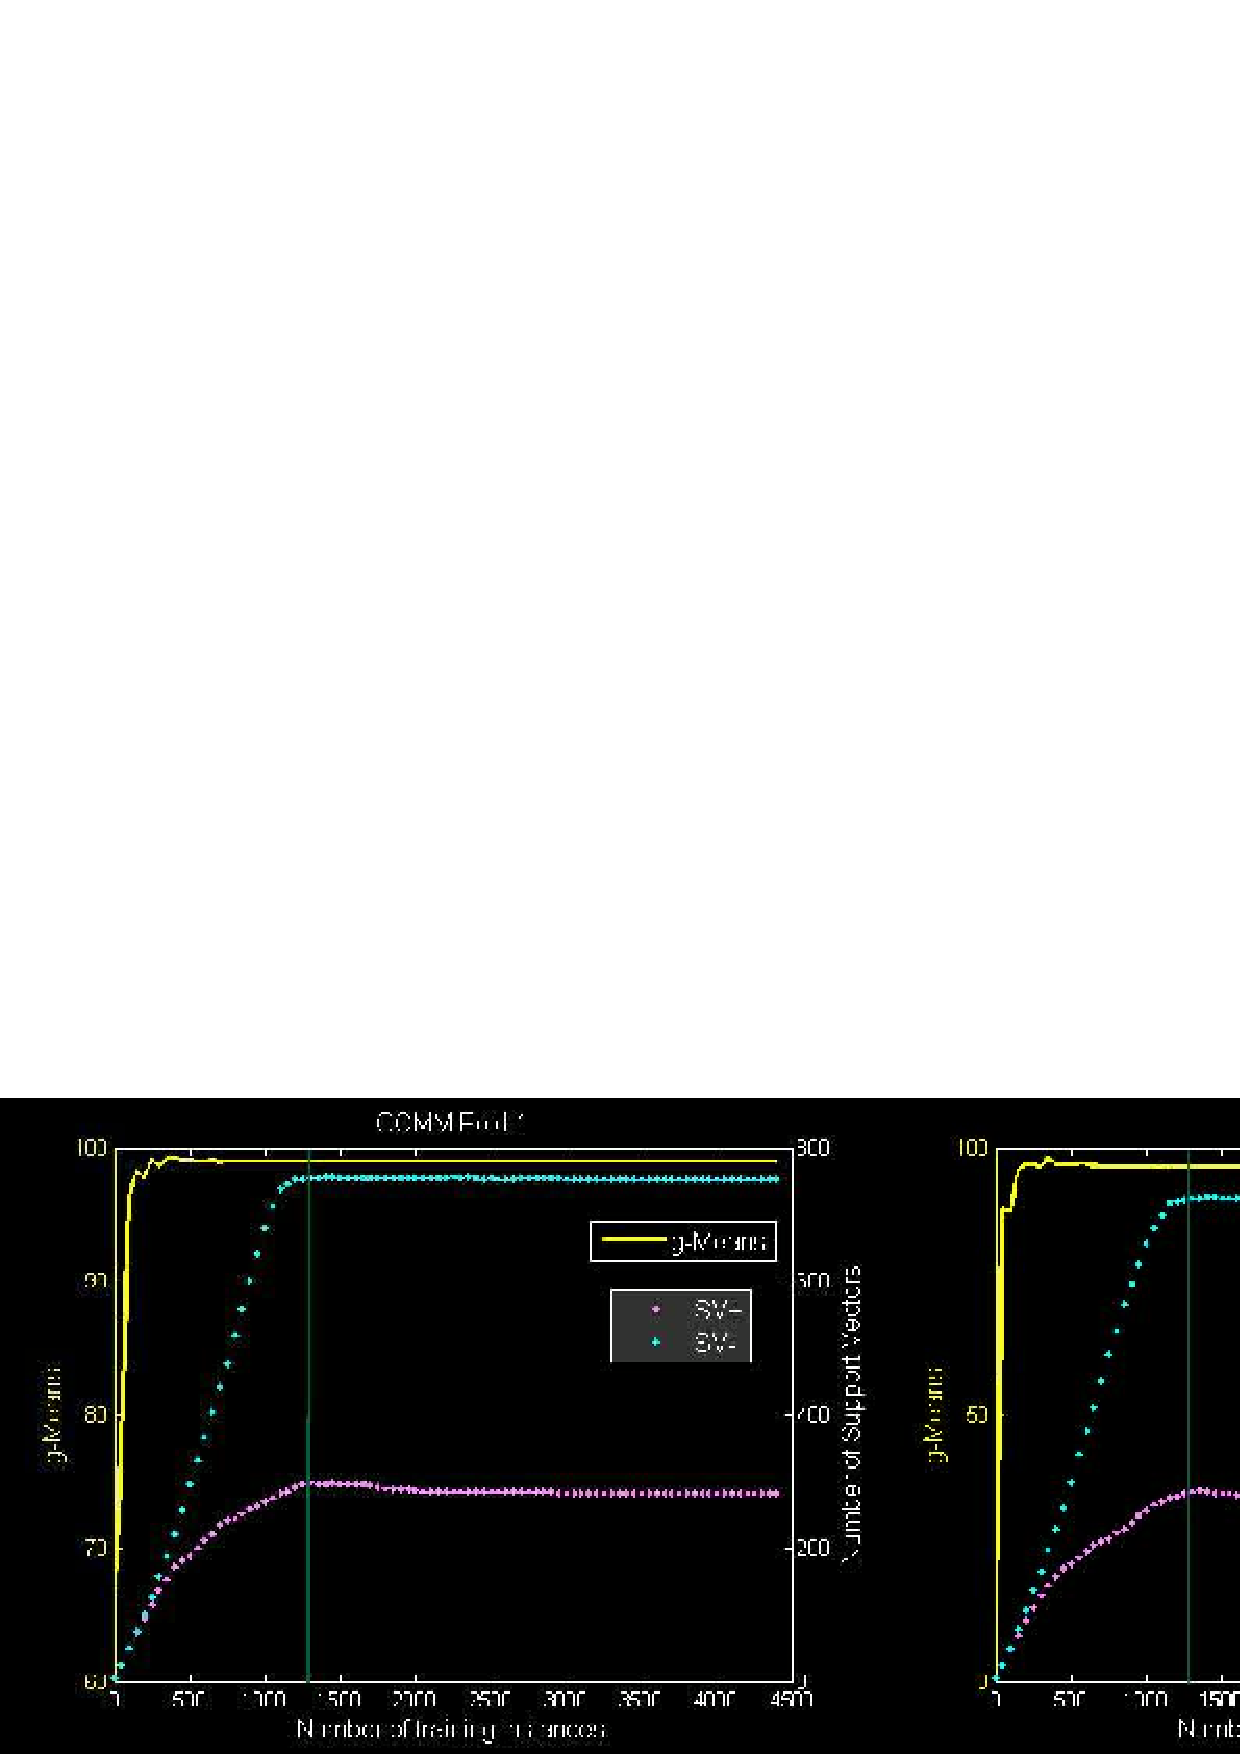
\includegraphics{Figures/lotb/comm.pdf}}
%    \caption{3-fold cross-validation results for the training set of the category COMM in CiteSeer dataset. Vertical lines correspond to early stopping points.}
%    \label{fig:comm}
%\end{figure}

%In order to analyze this method, we conducted a 3-fold cross-validation on one of the datasets (see Figure \ref{fig:comm}). In cross-validation, $2/3$ of the training set is used for training and the remaining $1/3$ is reserved as the hold-out dataset. Since the training set distribution is representative of the test set distribution, we believe that the algorithm's behavior would most likely be the same in the test set. As can be seen in Figure \ref{fig:comm}, in active learning setups, after using certain number of labeled training data, the number of support vectors saturates and  g-means levels off as well. Those graphs support the idea that the model does not change after the system observes enough informative samples. Further, adding more training data after this point does not make a remarkable change in the model and consequently in prediction performance. Notice that in Figure \ref{fig:comm} the vertical line indicates the suggested early stopping point and it is approximately equal in all three folds. As a result, we adopt the early stopping strategy of examining the number of support vectors in the entire training datasets without performing cross-validation.

\subsection{Performance Metrics}
Classification accuracy is not a good metric to evaluate classifiers in applications facing class imbalance problems.  SVMs have to achieve a tradeoff between maximizing the margin and minimizing the empirical error. In the non-separable case, if the misclassification penalty $C$ is very small, the SVM learner simply tends to classify every example as negative. This extreme approach maximizes the \textit{margin} while making no classification errors on the negative instances. The only error is the cumulative error of the positive instances which are already few in numbers. Considering an imbalance ratio of $99$ to $1$, a classifier that classifies everything as negative, will be $99\%$ accurate. Obviously,  such a scheme would not have any practical use as it would be unable to identify  positive instances.

For the evaluation of these results, it is useful to consider  several other prediction performance metrics such as g-means, AUC and PRBEP which are commonly used in imbalanced data classification. g-means \cite{Kubat_1997} is denoted as $g=\sqrt{sensitivity \cdot specificity}$ where sensitivity is the accuracy on the positive instances given as $True Pos./(True Pos.+False Neg.)$ and specificity is the accuracy on the negative instances given as $True Neg./(True Neg.+False Pos.)$.

The Receiver Operating Curve (ROC) displays the relationship between sensitivity and specificity at all possible thresholds for a binary classification scoring model, when applied to independent test data. In other words, ROC curve is a plot of the true positive rate against the false positive rate as the decision threshold is changed. The \textit{area under the ROC curve} (AUC) is a numerical measure of a model's discrimination performance and shows how successfully and correctly the model ranks and thereby separates the positive and negative observations. Since the AUC metric evaluates the classifier across the entire range of decision thresholds, it gives a good overview about the performance when the operating condition for the classifier is unknown or the classifier is expected to be used in situations with significantly different class distributions.

Precision Recall Break-Even Point (PRBEP) is another commonly used performance metric for imbalanced data classification. PRBEP is the accuracy of the positive class at the threshold where precision equals to recall. Precision is defined as $True Pos./(True Pos.+False Pos.)$ and recall is defined as $True Pos./(True Pos.+False Neg.)$


%\begin{table}[t!]
%\caption{Overview of the datasets.} \centering \small
%\begin{tabular}{l|l|r@{\hspace{2mm}}r@{\hspace{2mm}}r@{\hspace{2mm}}r|c c}
%\hline
%\multicolumn{2}{c|}{Dataset}&\#Feat.&\#Pos&\#Neg&Ratio&c&$\gamma$\\
%\hline\hline
%\multirow{5}{5mm}{\begin{sideways}\parbox{13mm}{Reuters}\end{sideways}}&Crude&8315&389&7381&19.0&2&1\\
%&Grain&8315&433&7337&16.9&2&1\\
%&Interest& 8315 &347&7423&21.4&1&2\\
%&Money-fx& 8315 &538&7232&13.4&1&0.5\\
%&Ship& 8315 &197&7573&38.4&1&0.5\\
%&Wheat& 8315 &212&7558&35.7&1&0.5\\
%\hline
%\multirow{5}{5mm}{\begin{sideways}\parbox{12mm}{CiteSeer}\end{sideways}}
%&AI& 6946 &1420&5353&4.3&50&0.1\\
%&COMM& 6946 &1252&5341&4.2&50&0.1\\
%&Crypt& 6946 &552&6041&11.0&50&0.1\\
%&DB& 6946 &819&5775&7.1&50&0.1\\
%&OS& 6946 &262&6331&24.2&50&0.1\\
%\hline
%\multirow{2}{5mm}{\begin{sideways}\parbox{8mm}{UCI}\end{sideways}}
%&Abalone-7& 9 &352&3407&9.7&100&0.01\\
%&Letter-A&16 &710&17290&24.4&10&0.01\\
%&Satimage&36&415&4020&9.69&50&0.001\\
%\hline
%\multicolumn{2}{c|}{USPS}& 256 &1232&6097&5.0&1000&2\\
%\hline
%\multicolumn{2}{c|}{MNIST-8}& 780 &5851&54149&9.3&1000&0.02\\
%\hline
%\end{tabular}
%\label{tbl:overview}
%\end{table}

%\subsection{Datasets}
%We study the performance of the algorithm on various benchmark real-world datasets. The overview of the datasets are given in Table \ref{tbl:overview}. The \emph{Reuters-21578} is a popular text mining benchmark dataset. We test the algorithms with 8 of the top 10 most populated categories of \emph{Reuters-21578}. We did not use categories `earn' and `acq' since their class imbalance ratios are not high enough. As a text dataset, we also used 5 categories from CiteSeer\footnote{http://citeseer.ist.psu.edu} data. We used 4 benchmark datasets from the popular UCI Machine Learning Repository as well. \emph{Letter} and \emph{satimage} are image datasets. The `letter A' is used as the positive class in \emph{letter} and `class 4' (damp grey soil) is used as positive class in \emph{satimage}. \emph{Abalone} is a biology dataset where the instances labeled as `class 7' are used to form the positive class. \emph{MNIST} and \emph{USPS} are OCR data of handwritten digits and `digit 8' is used as a positive class in \emph{Mnist}. \emph{Adult} is a census dataset to predict if the income of a person is greater than 50K based on several census parameters, such as age, education, marital status etc. The training set consists of 32,562 instances and the class imbalance ratio is 3. \emph{Waveform} is a popular artificial dataset used commonly in simulation studies. These datasets cover a wide range of data imbalance ratios.

\subsection{Experiments and Empirical Evaluation}
\label{lotb_experiments}
%We first conduct experiments to compare the performance of AL(random pool) strategy with the traditional active learning method, AL(full search). The results show that with the proposed method, we can make faster active learning without sacrificing any prediction performance. In the rest of the section, we refer to AL(random pool) as AL since it is the only active learning method that we used afterwards.

%\begin{figure}[b!]
%        \scalebox{0.47}{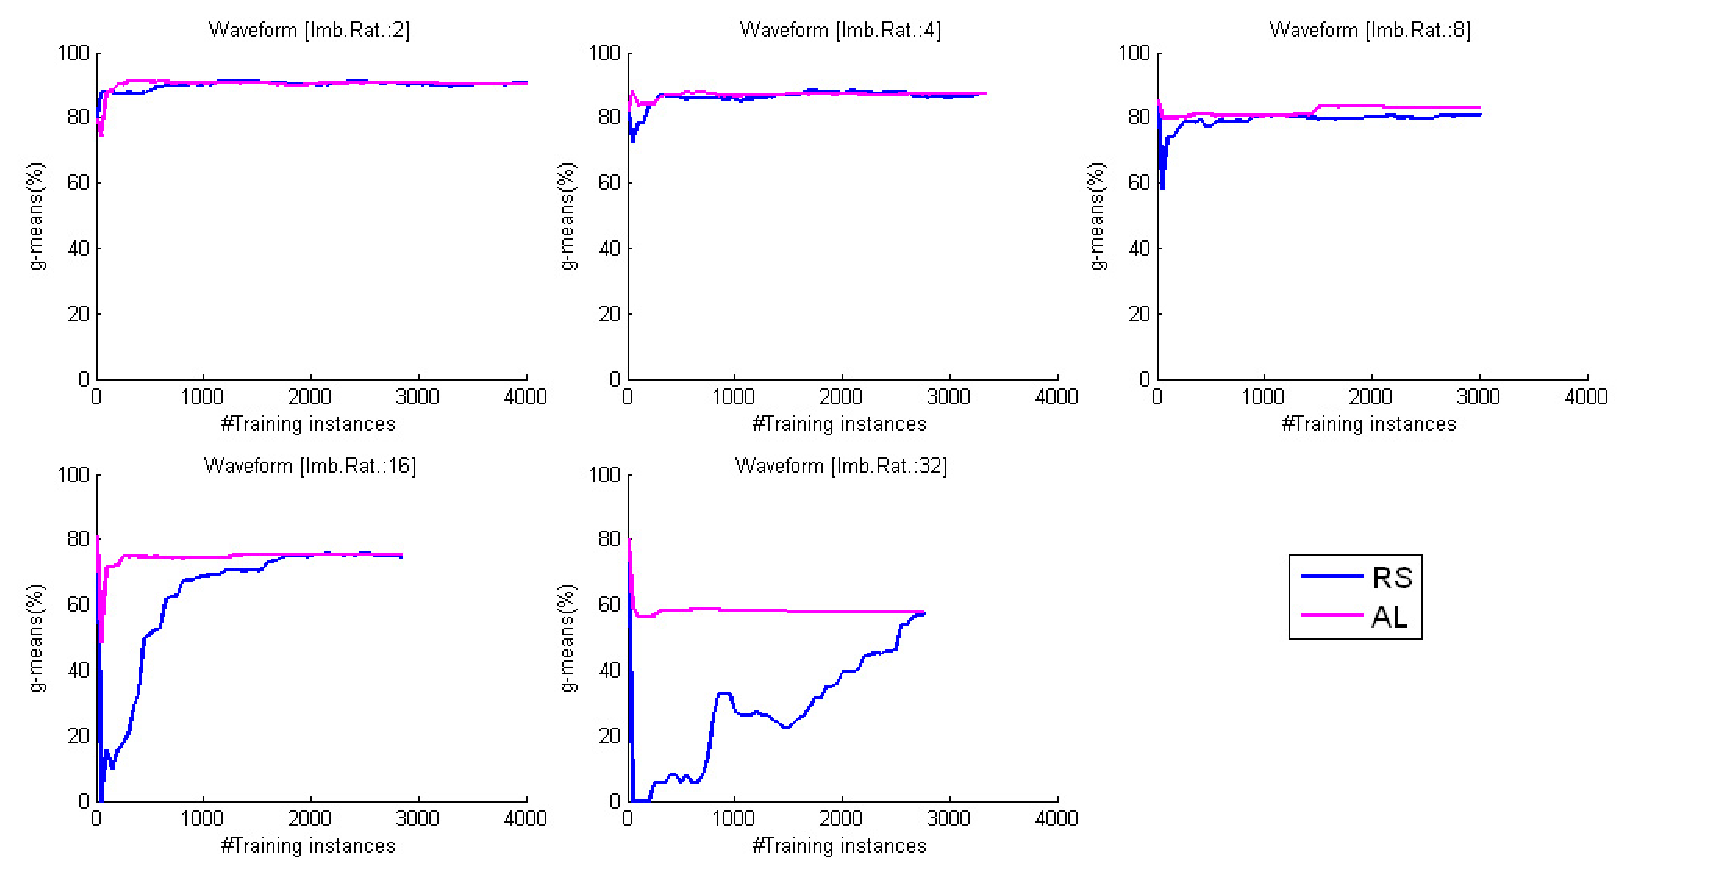
\includegraphics{Figures/lotb/wfall.eps}}
%    \caption{Comparison of g-means of AL and RS on the waveform datasets with different imbalance ratios (Imb.R.=2, 4, 8, 16, 32).}
%    \label{fig:wfall}
%\end{figure}
\begin{figure}[b!]
\begin{center}
\vspace{-4mm}
\subfigure {
\includegraphics[width=55mm]{Figures/lotb/adultall_1.jpg}
}
\subfigure {
\includegraphics[width=55mm]{Figures/lotb/adultall_2.jpg}
}\\
\vspace{-2mm}
\subfigure {
\includegraphics[width=55mm]{Figures/lotb/adultall_3.jpg}
}
\subfigure {
\includegraphics[width=55mm]{Figures/lotb/adultall_4.jpg}
}
 \caption{Comparison of PRBEP of AL and RS on the adult datasets with different imbalance ratios (Imb.R.=3, 10, 20, 30).}
    \label{fig:adultall}
\end{center}
\end{figure}


%In order to make a thorough analysis on the effect of AL(random pool) to imbalanced data classification, we examine its performance by varying class imbalance ratios using two performance metrics.
We study the performance of the algorithm on various benchmark real-world datasets, including MNIST, USPS, several categories of Reuters-21578 collection, five topics from CiteSeer, and three datasets from the UCI repository. The characteristics of the datasets are outlined in \cite{Ertekin2_2007}. In the experiments, an early stopping heuristic for active learning is employed, since it has been shown that active learning converges to the solution faster than the random sample selection method \cite{Ertekin2_2007}. A theoretically sound method to stop training is when the examples in the margin are exhausted. To check if there are still unseen training examples in the margin, the distance of the newly selected example is compared against the support vectors of the current model. If the new selected example by active learning (closest to the hyperplane) is not closer than any of the support vectors, it is concluded that the margin is exhausted. A practical implementation of this idea is to count the number of support vectors during the active learning training process. If the number of the support vectors stabilizes, it implies that all possible support vectors have been selected by the active learning method.

\begin{table*}[t!]\centering{
\caption{Comparison of g-means and AUC for AL and RS with entire training data (Batch).
SV ratios are given at the saturation point. Data efficiency corresponds to the percentage of training instances which AL processes to reach saturation.}
\begin{tabular}{l|l|r r|r r||r|r|c}
\hline
\multicolumn{2}{c|}{\multirow{2}{1cm}{Dataset}}
&\multicolumn{2}{c|}{g-means (\%)}
&\multicolumn{2}{c||}{AUC (\%)}
&Imb.&SV- /&\multirow{2}{12mm}{Data Efficiency}
\\
\cline{3-6}
\multicolumn{2}{c|}{}&Batch&AL&Batch&AL&Rat.&SV+\\
\hline\hline
\multirow{8}{1mm}{\begin{sideways}\parbox{12mm}{Reuters}\end{sideways}}
&Corn&85.55&86.59&99.95&99.95&41.9&3.13&11.6\%\\
&Crude&88.34&89.51&99.74&99.74&19.0&2.64&22.6\%\\
&Grain&91.56&91.56&99.91&99.91&16.9&3.08&29.6\%\\
&Interest&78.45&78.46&99.01&99.04&21.4&2.19&30.9\%\\
&Money-fx&81.43&82.79&98.69&98.71&13.4&2.19&18.7\%\\
&Ship&75.66&74.92&99.79&99.80&38.4&4.28&20.6\%\\
&Trade&82.52&82.52&99.23&99.26&20.1&2.22&15.4\%\\
&Wheat&89.54&89.55&99.64&99.69&35.7&3.38&11.6\%\\
\hline
\multirow{5}{1mm}{\begin{sideways}\parbox{12mm}{CiteSeer}\end{sideways}}
&AI&87.83&88.58&94.82&94.69&4.3&1.85&33.4\%\\
&COMM&93.02&93.65&98.13&98.18&4.2&2.47&21.3\%\\
&CRYPT&98.75&98.87&99.95&99.95&11.0&2.58&15.2\%\\
&DB&92.39&92.39&98.28&98.46&7.1&2.50&18.2\%\\
&OS&91.95&92.03&98.27&98.20&24.2&3.52&36.1\%\\
\hline
\multirow{3}{1mm}{\begin{sideways}\parbox{6mm}{UCI}\end{sideways}}
&Abalone-7&100.0&100.0&100.0&100.0&9.7&1.38&24.0\%\\
&Letter-A&99.28&99.54&99.99&99.99&24.4&1.46&27.8\%\\
&Satimage&82.41&83.30&95.13&95.75&9.7&2.62&41.7\%\\
\hline
\multicolumn{2}{c|}{USPS}&99.22&99.25&99.98&99.98&4.9&1.50&6.8\%\\
\hline
\multicolumn{2}{c|}{MNIST-8}&98.47&98.37&99.97&99.97&9.3&1.59&11.7\%\\
\hline
\end{tabular}
\label{tbl:AUC}

}
\end{table*}

As the first experiment, examples are randomly removed from the minority class in \emph{Adult} dataset to achieve different data imbalance ratios, comparing SVM-based active learning (AL) and random sampling (RS).\footnote{Here, the random process is assumed to be uniform; examples are selected with equal probability from the available pool.} \josh {I don't understand the following sentence} \seyda{Addressed.}  For brevity, AL with small pools is referred to as AL since the small pools heuristic is utilized for all active learning methods considered later. Comparisons of PRBEP in Figure \ref{fig:adultall} show an interesting behavior. As the class imbalance ratio is increased, AL curves display peaks in the early steps of the learning. This implies that by using an early stopping criteria AL can give higher prediction performance than RS can possibly achieve even after using all the training data. The learning curves presented in Figure \ref{fig:adultall} demonstrate that the addition of instances to a model's training after finding those most informative instances can be detrimental to the prediction performance of the classifier, since this may cause the model to suffer from overfitting. Figure \ref{fig:adultall} curves show that generalization can peak to a level above that can be achieved by using all available training data. In other words,it is possible to achieve better classification performance from a small informative subset of the training data than what can achieved using all available training data. This finding agrees with \cite{Schohn_2000} and strengthens the idea of applying an early stopping to active learning algorithms. \josh{say a few sentences why this may be the case? one can easily be surprised to learn that throwing away data can be a good thing.}\seyda{Added a few more sentences above and also a reference.}

For further comparison of the performance of the performance of a model built on all available data (Batch) and AL subject to early halting criteria, refer to Table~\ref{tbl:AUC}, comparing  the g-means and the AUC values for these two methods. The data efficiency column for AL indicates that by processing only a portion of the examples from the training set, AL can achieve similar or even higher generalization performance than that of Batch which sees all the training examples. Another important observation from Table \ref{tbl:AUC} is that support vector imbalance ratios in the final models are much less than the class imbalance ratios of the datasets. This confirms the discussion of Figure \ref{fig:alimbshade}. The class imbalance ratio within the margins are much less than the class imbalance ratio of the entire data and active learning can be used to reach those informative examples which most likely become support vectors without seeing all the training examples.


\begin{figure}[t!]
    \centering
        \scalebox{0.4}{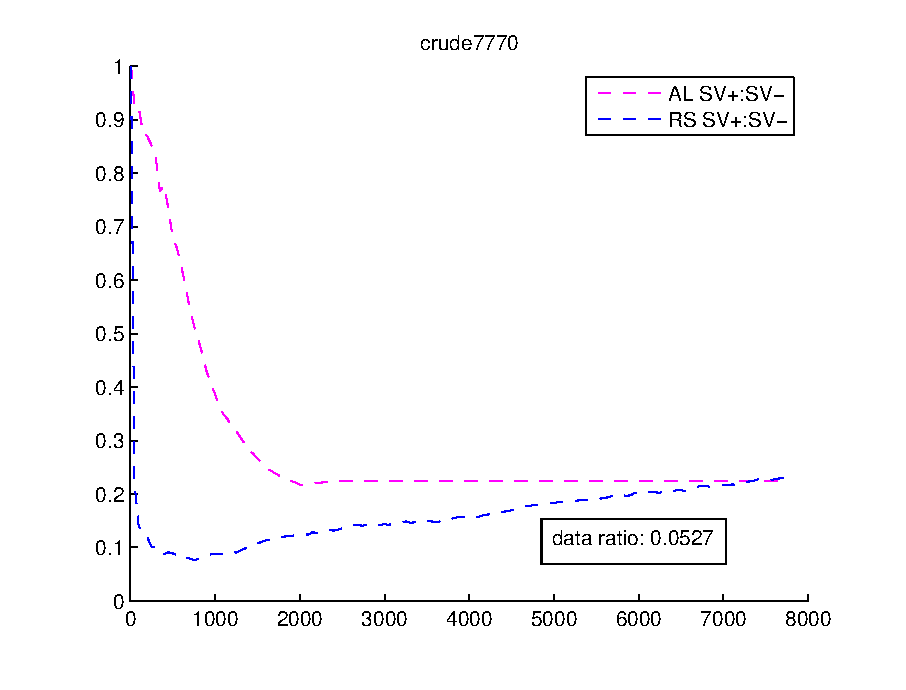
\includegraphics{Figures/lotb/cruderatio.eps}}
    \caption{Support Vector ratios in AL and RS}
    \label{cruderatio}
\end{figure}

Figure \ref{cruderatio} investigates how the number of support vectors changes when presented with examples selected according to  AL and RS. Because the base rate of the dataset gathered by RS approaches that of the example pool, the support vector imbalance ratio quickly approaches the data imbalance ratio. As learning continues, the learner should gradually see all the instances within the final margin and the support vector imbalance ratio decreases. At the end of training with RS, the support vector imbalance ratio is the data imbalance ratio within the margin. The support vector imbalance ratio curve of AL is drastically different than RS. AL intelligently picks the instances closest to the margin in each step. Since the data imbalance ratio within the margin is lower than data imbalance ratio, the support vectors in AL are more balanced than RS during learning. Using AL, the model saturates by seeing only 2000 (among 7770) training instances and reaches the final support vector imbalance ratio. Note that both methods achieve similar support vector imbalance ratios when learning finishes, but AL achieves this in the early steps of the learning.

It is also interesting to consider the performance of active learning as a selection heuristic in light of more conventional sampling strategies. Here, AL is compared to traditional under-sampling of the majority class (US), and an oversampling method (SMOTE), both examples of resampling techniques which require preprocessing. It has been shown that oversampling at random does not help to improve prediction performance \cite{Japkowicz_2002} therefore a more complex oversampling method is required.  Synthetic Minority Oversampling Technique (SMOTE) oversamples the minority class by creating synthetic examples rather than with replacement. The $k$ nearest positive neighbors of all positive instances are identified and synthetic positive examples are created and placed randomly along the line segments joining the $k$ minority class nearest neighbors.


For additional comparison, the method of assigning different costs (DC) to the positive and negative classes as the misclassification penalty parameter is examined. For instance, if the imbalance ratio of the data is 19:1 in favor of the negative class, the cost of misclassifying a positive instance is set to be 19 times greater than that of misclassifying a negative one. We use the online SVM package LASVM\footnote{Available at \texttt{http://leon.bottou.org/projects/lasvm}} in all experiments. Other than the results of the methods addressing the class imbalance problem, the results of Batch algorithm with the original training set are provided to form a baseline. LASVM is run in random sampling mode for US, SMOTE and DC.

\begin{figure*}[t!]
    \hspace{-5mm}
        \scalebox{0.48}{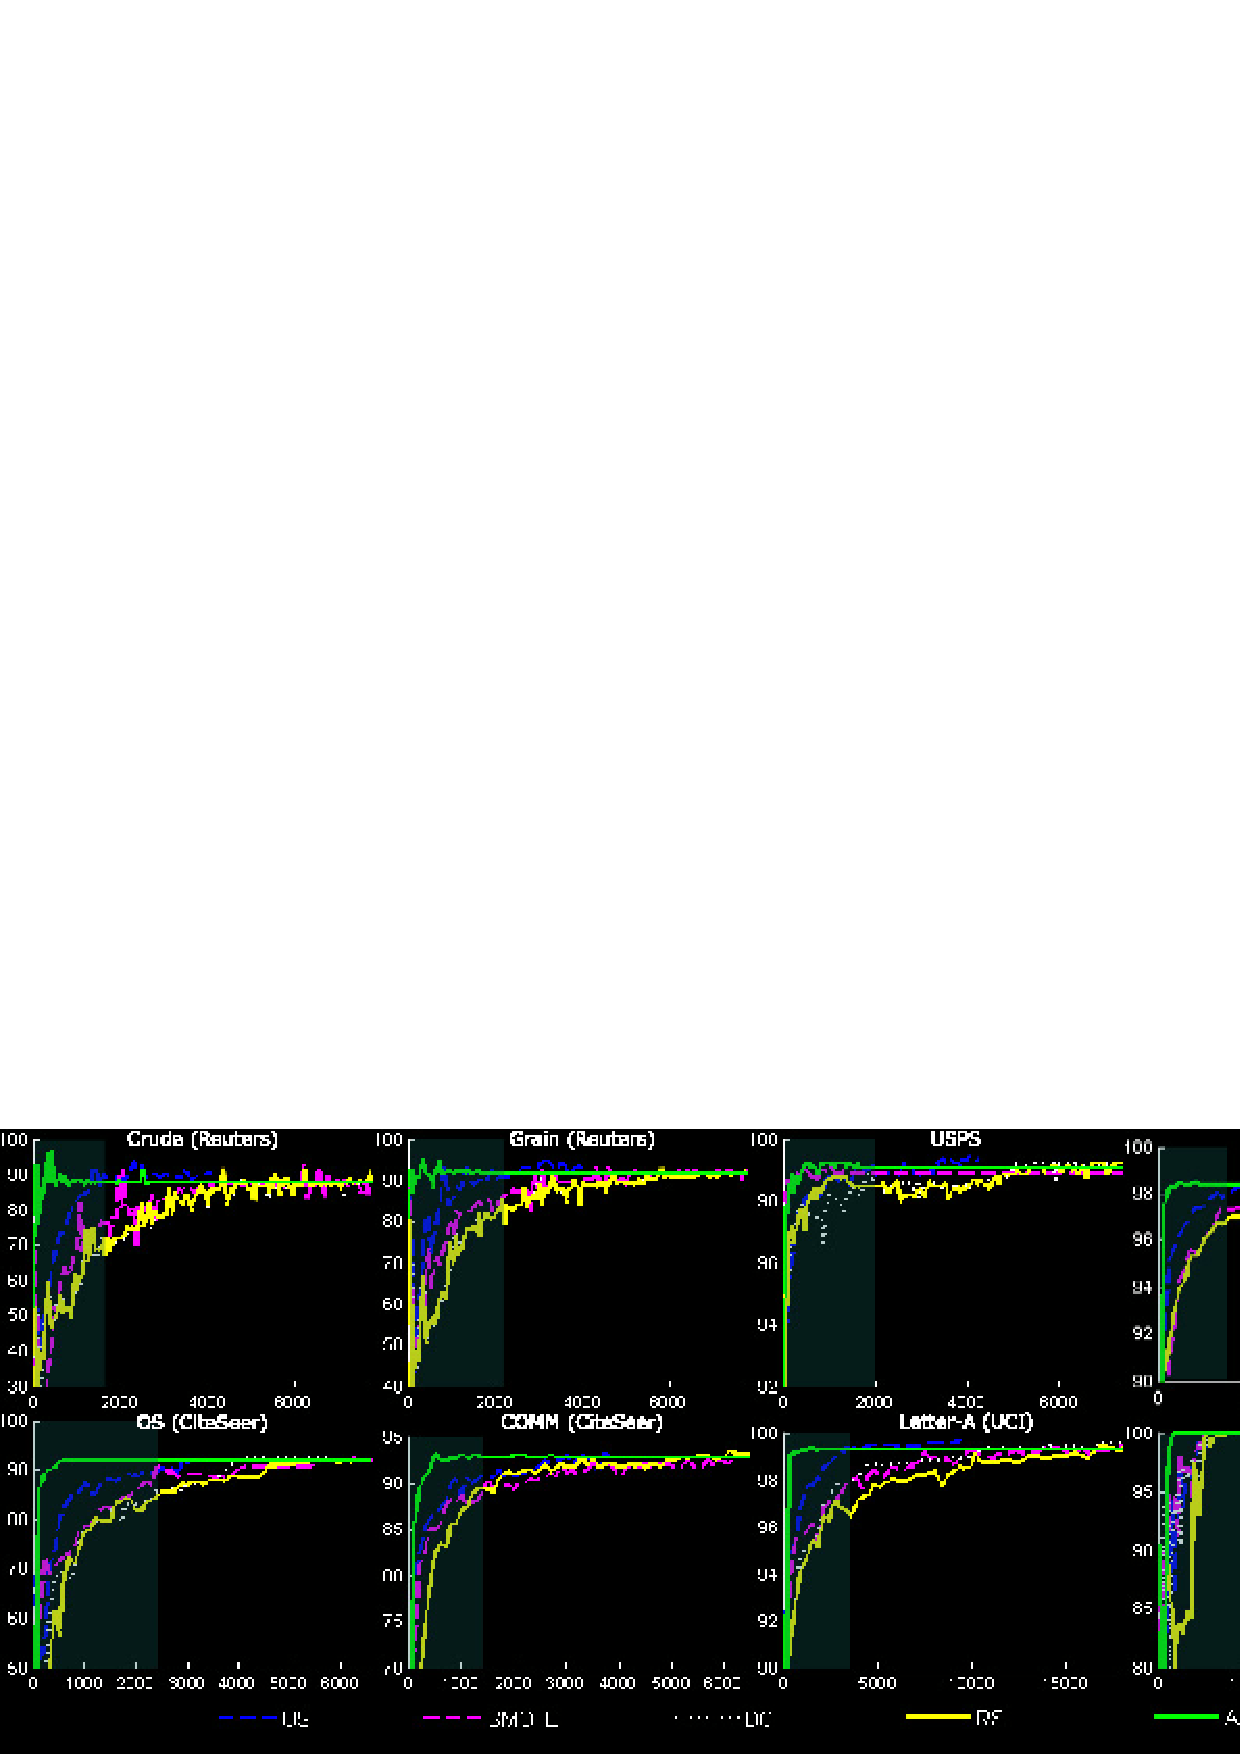
\includegraphics{Figures/lotb/big8.pdf}}
    \caption{Comparisons of g-means. The right border of the shaded area corresponds to the early stopping point.}
    \label{eightgraphs}
\end{figure*}


We present the comparisons of the methods for g-means performance metric for several datasets in Figure \ref{eightgraphs}. The right border of the shaded pink area is the place where the aforementioned early stopping strategy is applied.  The curves in the graphs are averages of 10 runs. For completeness, all  AL experiments were allowed to continue to select examples until exhaustion, bypassing any early stopping.  Table \ref{tbl:results} presents the PRBEP of the methods and the total running times of the SMOTE and AL on 18 benchmark and real-world datasets. The results for active learning in Table \ref{tbl:results} depict the results in the early stopping points. The results for the other methods in Table \ref{tbl:results} depict the values at the end of the curves--- when trained with the entire dataset--- since those methods do not employ any early stopping criteria. We did not apply early stopping criteria to the other methods because, as observed from Figure \ref{eightgraphs}, no early stopping criteria would achieve a comparable training time with of AL's training time without a significant loss in their prediction performance based on convergence time. The other methods converge to similar levels of g-means when nearly all training instances are used, and applying an early stopping criteria would have little, if any, effect on their training times.

\begin{table*}[b!]\centering{
\caption{Comparison of PRBEP and training time. }\small
\begin{tabular}{l|l|r r r r r|r r}
\hline
\multicolumn{2}{c|}{Metric}&\multicolumn{5}{c|}{PRBEP}&\multicolumn{2}{c}{Training time (sec.)}\\
\hline
\multicolumn{2}{c|}{Dataset}&Batch&US&SMOTE&DC&AL&SMOTE&AL\\
\hline
\hline
\multirow{8}{5mm}{\begin{sideways}\parbox{13mm}{Reuters}\end{sideways}}
&Corn&91.07&78.57&91.07&89.28&89.29&87&16\\
&Crude&87.83&85.70&87.83&87.83&87.83&129&41\\
&Grain&92.62&89.93&91.44&91.94&91.94&205&50\\
&Interest&76.33&74.04&77.86&75.57&75.57&116&42\\
&Money-fx&73.74&74.30&75.42&75.42&76.54&331&35\\
&Ship&86.52&86.50&88.76&89.89&89.89&49&32\\
&Trade&77.77&76.92&77.77&77.78&78.63&215&38\\
&Wheat&84.51&81.61&84.51&84.51&85.92&54&25\\
\hline
\multirow{5}{5mm}{\begin{sideways}\parbox{12mm}{CiteSeer}\end{sideways}}
&AI&78.80&80.68&78.99&78.79&79.17&1402&125\\
&COMM&86.59&86.76&86.59&86.59&86.77&1707&75\\
&CRYPT&97.89&97.47&97.89&97.89&97.89&310&19\\
&DB&86.36&86.61&86.98&86.36&86.36&526&41\\
&OS&84.07&83.19&84.07&84.07&84.07&93&23\\
\hline
\multirow{3}{5mm}{\begin{sideways}\parbox{6mm}{UCI}\end{sideways}}
&Abalone-7&100.0&100.0&100.0&100.0&100.0&16&4\\
&Letter-A&99.48&96.45&99.24&99.35&99.35&86&3\\
&Satimage&73.46&68.72&73.46&73.93&73.93&63&21\\
\hline
\multicolumn{2}{c|}{USPS}&98.44&98.44&98.13&98.44&98.75&4328&13\\
\hline
\multicolumn{2}{c|}{MNIST-8}&97.63&97.02&97.74&97.63&97.74&83,339&1,048\\
\hline

\end{tabular}
\label{tbl:results}
}
\end{table*}

Since AL involves discarding some instances from the training set, it can be perceived as a type of under-sampling method. Unlike traditional US, which discards majority samples randomly, AL performs an intelligent search for the most informative ones adaptively in each iteration according to the current hyperplane. Datasets where class imbalance ratio is high such as \emph{corn}, \emph{wheat}, \emph{letter} and \emph{satimage} observe significant decrease in PRBEP of US (see Table 3). Note that US's under-sampling rate for the majority class in each category is set to the same value as the final support vector ratio which AL reaches in the early stopping point and RS reaches when it sees the entire training data. Although the class imbalance ratio provided to the learner in AL and US are the same, AL achieves significantly better PRBEP performance metric than US. The Wilcoxon signed-rank test (2-tailed) reveals that the zero median hypothesis can be rejected at the significance level 1\% (p=0.0015), implying that AL performs statistically better than US in these 18 datasets. These results reveal the importance of using the informative instances for learning.

%Table \ref{tbl:rankresults} presents the rank of PRBEP prediction performance of the five approaches in a variety of datasets. The values in bold correspond to the cases where AL wins and it's clear that winning cases are very frequent for AL (12 out of 18 cases). The average rank also indicates that AL achieves the best PRBEP among the five methods. SMOTE and DC achieve higher PRBEP than the Batch algorithm. The loss of information when undersampling the majority class affects US's prediction performance.

Table \ref{tbl:results} gives the comparison of the computation times of the AL and SMOTE. Note that SMOTE requires significantly long preprocessing time which dominates the training time in large datasets, e.g., MNIST-8 dataset. The low computation cost, scalability and high prediction performance of AL suggest that AL can efficiently handle the class imbalance problem.
